\documentclass[11pt]{article}

\usepackage{amsmath,amssymb,amsthm,amsfonts,amscd,tikz} %usual symbols, theorems, etc
\usepackage{tikz-cd} %diagrams
\usepackage{multicol} %columns
\usepackage{enumerate} %lists
\usepackage{hyperref} %links, references
\usepackage{aliascnt} %copies counters but with new labels --- for autoref
\usepackage{graphicx} %pictures
\usepackage{subcaption} %subfigures - use minipage
\usetikzlibrary{arrows,matrix,calc,decorations.pathmorphing} %curved arrows
\usepackage{mathabx} %more symbols
\usepackage{mathrsfs} %super curly letters
\usepackage{bbm} %quaternions
%\usepackage{microtype} %supposedly makes things nicer, ask Peter
\usepackage[margin=1in]{geometry} %margins
\usepackage{wrapfig} %wraps figures/tables in text
\usepackage{cite} %citations
\usepackage{sage} %new! sage tex package



%GENERAL SYMBOLS
\newcommand{\BB}[1]{\mathbb{#1}} %bold face
\newcommand{\script}[1]{\mathcal{#1}} %curvy
\newcommand{\curly}[1]{\mathscr{#1}} %extra curvy
\newcommand{\cat}[1]{\textbf{\emph{#1}}} %bold
\renewcommand{\frak}[1]{\mathfrak{#1}} %gothic
\newcommand{\del}[1]{\frac{\partial}{\partial{#1}}} %single derivative vector d/dx
\newcommand{\ddel}[2]{\frac{\partial{#1}}{\partial{#2}}} %dy/dx
\newcommand{\floor}[1]{{\lfloor #1 \rfloor}} %flooor
\newcommand{\free}[1]{\left\langle#1\right\rangle} %nice brackets

%SPECIFIC SYMBOLS
\newcommand{\CC}{\BB{C}}
\newcommand{\RR}{\BB{R}}
\newcommand{\NN}{\BB{N}}
\newcommand{\QQ}{\BB{Q}}
\newcommand{\ZZ}{\BB{Z}}
\newcommand{\PP}{\BB{P}}
\renewcommand{\AA}{\BB{A}} %\AA is a non-ascii acented A, weird
\newcommand{\HH}{\BB{H}}
\newcommand{\DD}{\BB{D}}
\newcommand{\TT}{\BB{T}}
\newcommand{\FF}{\BB{F}}
\newcommand{\RP}{\RR\PP}
\newcommand{\CP}{\CC\PP}
\renewcommand{\SS}{\BB{S}} %\SS is a silly non-ascii letter "SS".
\newcommand{\st}{\colon}
\newcommand{\im}{\operatorname{Im}}
\newcommand{\re}{\operatorname{Re}}
\newcommand{\Int}{\operatorname{Int}}
\newcommand{\diam}{\operatorname{diam}}
\newcommand{\rank}{\operatorname{rank}}
\newcommand{\codim}{\operatorname{codim}}
\newcommand{\nullity}{\operatorname{nullity}}
\newcommand{\diag}{\operatorname{diag}}
\newcommand{\supp}{\operatorname{Supp}}
\newcommand{\Aut}{\operatorname{Aut}}
\newcommand{\sgn}{\operatorname{sign}}
\newcommand{\sing}{\operatorname{sing}}
\newcommand{\tr}{\operatorname{tr}}
\newcommand{\GL}{\operatorname{GL}}
\newcommand{\SL}{\operatorname{SL}}
\newcommand{\PSL}{\operatorname{PSL}}
\newcommand{\PGL}{\operatorname{PGL}}
\newcommand{\Pic}{\operatorname{Pic}}
\newcommand{\Gal}{\operatorname{Gal}}
\newcommand{\chr}{\operatorname{char}}
\newcommand{\ord}{\operatorname{ord}}
\newcommand{\res}{\operatorname{res}}
\newcommand{\Hom}{\operatorname{Hom}}

%first theorem style
\newtheorem{thmc}{pleasedontusethistheoremenvironment}[section]

%builds a theorem environment with
%theoremstyle as first arg
%theorem reference as second
%printed name of theorem as 3rd
\makeatletter
\newcommand{\newlabeledtheoremenv}[3][plain]{
	\theoremstyle{#1}
	\newaliascnt{#2}{thmc} %theorem has it's own counter
	\newtheorem{#2}[#2]{#3}
	\aliascntresetthe{#2}
	\@namedef{#2autorefname}{#3}%
}
\makeatother

\newlabeledtheoremenv[plain]{thm}{Theorem}
\newlabeledtheoremenv[plain]{lem}{Lemma}
\newlabeledtheoremenv[definition]{rem}{Remark}
\newlabeledtheoremenv[plain]{prop}{Proposition}
\newlabeledtheoremenv[plain]{cor}{Corollary}
\newlabeledtheoremenv[definition]{defn}{Definition}
\newlabeledtheoremenv[definition]{ex}{Example}
\newlabeledtheoremenv[plain]{conj}{Conjecture}
\newlabeledtheoremenv[definition]{quest}{Question}
\newlabeledtheoremenv[definition]{note}{Note}
\newlabeledtheoremenv[definition]{fact}{Fact}


\theoremstyle{plain}
\newtheorem*{claim}{Claim}
\theoremstyle{remark}
\newtheorem*{reason}{Reason}

%page style, title page, custom variables
\newcommand{\mytitle}{Modular Curves}
\newcommand{\myauthor}{Travis Scholl}
\newcommand{\myemail}{tscholl2@uw.edu}
\date{February 11 2014}


\begin{document}
\title{\bfseries \mytitle}
\author{\sc \myauthor }
\maketitle

\section{Moduli Problems}

A \emph{moduli problem} is basically a way to parametrize a family of geometric objects to study some properties. We will be interested in \emph{moduli spaces} which we will use for the parametrization.

\begin{ex}\label{lineparam}
Consider the set of lines through the origin in $\RR^2$. Each is of the form $ax+by=0$ for some $a,b\in\RR$. Moreover, two lines agree if and only if their coefficients are a multiple of each other. This means there is a bijection between lines through the origin in $\RR^2$ and $\PP^1(\RR)$.

Moreover, this is a nice parameterization because lines through the origin in $\QQ^2$ are parametrized by $\PP^1(\QQ)$ which can be thought of as the rational points on $\PP^1(\RR)$. So there is a natural map from lines in $\QQ^2$ to lines in $\RR^2$ which corresponds with the map $\PP^1(\QQ) \to \PP^1(\RR)$.

Preview of whats to come: imagine a functor from $\cat{Fields}$ to $\cat{Set}$ by taking a field $k$ to all lines through the origin in $A^2_k$. What we said above is similar to saying this functor is represented by $\PP^1_k$.
\end{ex}

\section{Elliptic Curves as Lattices}

This section can be summarized by the following.
\begin{thm}
	There is an equivalence of categories between compact Riemann surfaces, function fields, and irreducible algebraic curves.
\end{thm}
\begin{proof}
	For compact Riemann surfaces to function fields see \cite[Chapter 1 Section 3 Proposition 1.95]{dessins}. The hardest part is showing there exist non-constant meromorphic functions on a arbitrary compact Riemann surface. For function fields and algebraic curves see \cite[Chapter 1 Section 6 Corollary 6.12]{hartshorne}
\end{proof}

\begin{note}
	Here an algebraic curve is a nonsingular projective variety of dimension $1$ over $\CC$ with dominant morphisms. Basically we need to remove trivial maps in each category.
\end{note}

We will specialize to subcategories of complex tori and elliptic curves.

\subsection{Objects}

Recall the identification of complex elliptic curves $E/\CC$ with complex tori $\CC/\Lambda$ for a lattice $\Lambda\subseteq\CC$. For example see \cite[Chapter III Section 3]{milne} or \cite[Chapter 1 Section 4]{diamondshurman}.

The main points are summarized here.
\begin{enumerate}[$\bullet$]
	\item Given a lattice (free $\ZZ$-submodule of rank $2$) $\Lambda\subseteq\CC$, the field of meromorphic functions on $\CC/\Lambda$ is $\CC(\wp,\wp')$ where $\wp$ is the Weierstrass $\wp$-function for $\Lambda$ given by $z\mapsto \sum_{\lambda\in L\setminus\{0\}} \left(\frac{1}{(z-\lambda)^2} - \frac{1}{\lambda^2}\right) + \frac{1}{z^2}$. %or equivalently $z\mapsto \frac{1}{z^2} + \sum_{k\geq 1}(2k+1)G_{2k+2}(\Lambda)z^n$ and $G_k(\Lambda) = \sum_{\omega\in\Lambda\setminus\{0\}}\frac{1}{\omega^{k}}$.

	\item The Wierstrass $\wp$-function satisfies
	$$
		\left(\frac{1}{2}\wp_{\Lambda}'\right)^2 = \wp^3 + a\wp + b
	$$
	where $a = -15 \sum_{\lambda\in L\setminus\{0\}}\frac{1}{\lambda^4}$ and $b = -35 \sum_{\lambda\in L\setminus\{0\}} \frac{1}{\lambda^6}$.

	\item The cubic equation $y^2 = x^3 + ax + b$ (with $a$,$b$ as above) is non-singular and thus defines a complex elliptic curve $E_{\Lambda}$.

	\item There is a map $\varphi:\CC/\Lambda \to E_{\Lambda}$ given by $z+\Lambda \mapsto \left(\wp(z),\frac{1}{2}\wp'(z)\right)$. This is an isomorphism as compact Riemann surfaces, nonsingular projective curves (note they have the same function fields), and also as algebraic groups. The last one can be shown by writing out $\wp(z_1+z_2)$ as a rational function in $\wp,\wp'$ applied to $z_1,z_2$, then show $z_1+z_2+z_3\in\Lambda \Rightarrow \varphi(z_1),\varphi(z_2),\varphi(z_3)$ are colinear.
\end{enumerate}
This shows every lattice corresponds to a complex elliptic curve. One can show this process is surjective [see just about any reference, including \cite{diamondshurman}], i.e. every elliptic curve corresponds to an elliptic curve given by some (non-unique!) lattice.

\subsection{Morphisms}

First we need to know what the morphisms of Tori look like.

\begin{thm}
	Suppose $\varphi:\CC/\Lambda \to \CC/\Lambda'$ is a meromorphic function sending $0\mapsto 0$. Then $\varphi$ is induced by the map $z\mapsto mz$ for some $m\in\CC$ such that $m\Lambda\subseteq \Lambda'$. In particular, such a map is an isomorphism if and only if $m\Lambda = \Lambda'$.
\end{thm}
\begin{proof}(See \cite[Chapter 1 Section 3]{diamondshurman} or Ralph's notes)
	\hfill

	Consider the following diagram.
	$$
	\begin{tikzcd}
		\CC \rar{\psi}\dar{\pi} & \CC\dar{\pi'}
		\\
		\CC/\Lambda \rar{\varphi} & \CC/\Lambda'
	\end{tikzcd}
	$$
	The map $\psi$ comes from lifting the map $\varphi\circ\pi$ which is possible as $\CC$ is the universal covering space of $\CC/\Lambda'$. We can choose $\psi$ such that $\psi(0)=0$ by the hypothesis on $\varphi$. Now $\psi$ is a priori continuous, but we can show it is analytic by noting that $\pi,\pi'$ are locally conformal.

	Fix some $\lambda\in\Lambda$ and consider the map $f(z) = \psi(z+\lambda) - \psi(z)$. Clearly this is an entire analytic function on $\CC$ and moreover
	\begin{align*}
		(\pi'\circ f)(z)
		&=
		\pi'\circ\psi(z+\lambda) - \pi'\circ\psi(z)
		\\
		&=
		\varphi\circ\pi(z+\lambda) - \varphi\circ\pi(z)
		\\
		&= 0
	\end{align*}
	Hence $\im f\subseteq \Lambda'$. Since this is a discrete set $f$ is constant and therefore
	$$
	f'(z) = 0 \Rightarrow \psi'(z+\lambda) = \psi'(z).
	$$
	In particular this shows $\psi'$ is $\Lambda$-periodic hence bounded. But $\psi'$ is an entire analytic function, so by Louivilles Theorem $\psi' = m$ for some $m\in\CC$. Because we constructed $\psi$ so that $0\mapsto 0$, so $\psi(z) = mz$.

	From the commutativity of the diagram we have $\psi(\Lambda) = m\Lambda\subseteq\Lambda'$.
\end{proof}

\begin{note}
	Dropping the requirement on $0$ will mean analytic maps are of the form $mz+b$. These are \emph{homotheties}. What this means though, is that any map of Tori which fixes $0$ is automatically a group homomorphism. This carries over to Elliptic curves as well!
\end{note}

In summary we now have a concrete space of elliptic curves to work with.

\begin{thm}\label{latticetori}
	Let $\script{L}$ be the space of lattices. Then the map $\Lambda\mapsto \CC/\Lambda$ induces a bijection $\script{L}/\CC^\ast \to \{\CC/\Lambda\}/\approx$ where $\approx$ is complex isomorphism of Tori.
\end{thm}

Because of our equivalence of categories this means
\begin{thm}
	$\CC/\Lambda_1 \cong \CC/\Lambda_2$ if and only if $E_{\Lambda_1}\cong E_{\Lambda_2}$. Moreover, all the relevant structure (e.g. group structure) is preserved as well.
\end{thm}



\section{Preliminaries}

There is a left action of $\SL_2(\ZZ)$ on the upper half plane $\HH$ given by
$$
\begin{pmatrix}a & b \\ c & d\end{pmatrix} \cdot \tau = \frac{a\tau+b}{c\tau+d}.
$$

%\begin{defn}[Fourier Series]
%	Given a function $f(\tau)$ with period $1$ on $\HH$, the \emph{Fourier series $F$ of $f$} is the unique function on $\DD$ by the
%	$$
%	\begin{tikzcd}
%		\HH \dar[swap]{e^{2\pi i \tau}}\rar{f} & \CC
%		\\
%		\DD \urar[swap]{F}
%	\end{tikzcd}
%	$$
%	we will represent $F$ by $f(q)$ where $q = e^{2\pi i \tau}$. This makes sense because $f$ is constant on the fibers of the covering map $e^{2\pi i \tau}$.
%\end{defn}
\noindent
Define
$$
	\Gamma(1) := \SL_2(\ZZ)
$$
$$
	\Gamma_0(N) := \left\{\begin{pmatrix}a & b \\ c & d\end{pmatrix}\in\SL_2(\ZZ) \mid  c\equiv 0\mod{N}\right\}.
$$
$$
	\Gamma_1(N) := \left\{\begin{pmatrix}a & b \\ c & d\end{pmatrix}\in\SL_2(\ZZ) \mid  c\equiv 0\mod{N}, a\equiv d\equiv 1\mod{N}\right\}.
$$
we will see exactly why we these restrictions are exactly what we need.


Now define quotients $Y(1),Y_0(N),Y_1(N)$ as $\Gamma(1)\backslash\HH,\Gamma_0(N)\backslash\HH,\Gamma_1(N)\backslash\HH$. Since the action is nice (besides a few odd points), these are complex manifolds. However, they are not compact.

Define $X(1),X_0(N),X_1(N)$ in the same way using the \emph{extended upper half plane} $\HH^* = \HH\cup\QQ\cup\{\infty\}$ instead of $\HH$. These spaces are compact, and usually referred to as the compactifications of the $Y$ spaces. The equivalence classes of $\QQ\cup\{\infty\}$ are called \emph{cusps}. It is not hard to show the $X$ spaces have finitely many cusps. It will follow from a few facts such as the natural map $X_0(N) \to X(1)$, $X(1)$ has one cusp, and $[\SL_2(\ZZ)\st\Gamma_0(N)]$ is finite.

\begin{note}
	Some people study much more general spaces by using more general subgroups $\Gamma\subseteq\SL_2(\ZZ)$.
\end{note}

\begin{note}
	Points in $\HH^*$ with non-trivial isotropy subgroup are called \emph{elliptic points}. It turns out elliptic points always have finite cyclic isotropy subgroups. Note $i,\rho = e^{2\pi i/3}$ are the only elliptic points in $Y_1(1)$. In general, there is only a finite number of elliptic points and they are only possibly in the preimage of $i,\rho$ under $X \to X_0(1)$ for any of the $X$ spaces.
\end{note}

One can show all the $X$ spaces are compact Riemann surfaces. The charts are obvious except for at cusps and elliptic points, here you use various power maps. Also the topology is similar to the standard ones except at cusps. A base is given by the circles (Euclidean) tangent to $\RR$. This is equivalent to taking the usual topology on $\HH\cup\{\infty\}$ and then applying $\SL_2(\ZZ)$ to all the open subsets to get open subsets of $\QQ$ points.

It's fun to draw pictures of the \emph{fundamental domain} of these regions. For example the following sage code produces the fundamental domains shown in \autoref{fund_domains}.
\begin{sagecode}
\begin{sagecell}
X0_1 = FareySymbol(Gamma0(1)).fundamental_domain(tesselation=None,show_pairing=True)
X0_3 = FareySymbol(Gamma0(3)).fundamental_domain(tesselation=None,show_pairing=True)
X0_11 = FareySymbol(Gamma0(11)).fundamental_domain(tesselation=None,show_pairing=True)
X0_23 = FareySymbol(Gamma0(23)).fundamental_domain(tesselation=None,show_pairing=True)
\end{sagecell}
\end{sagecode}
\begin{figure}
	\begin{subfigure}{.5\linewidth}
	\centering
	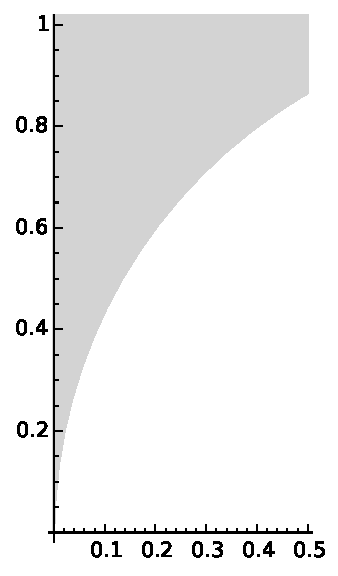
\includegraphics[width=0.6\linewidth]{X0_1.pdf}
	\caption{$X_0(1)$\label{X0_1.svg}}
	\end{subfigure}
	\begin{subfigure}{.5\linewidth}
	\centering
	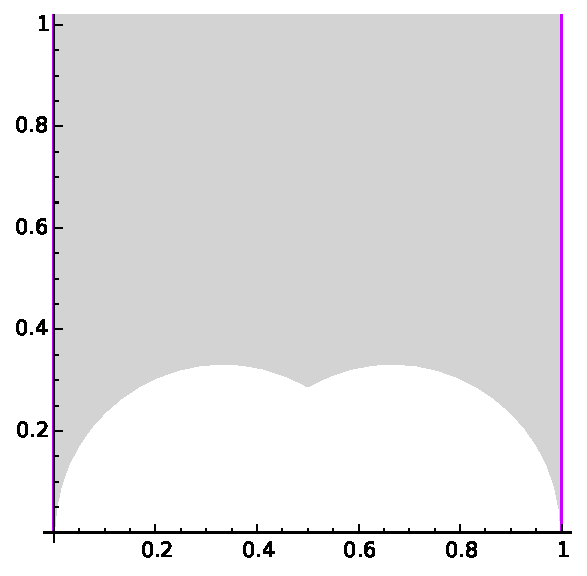
\includegraphics[width=1\linewidth]{X0_3.pdf}
	\caption{$X_0(3)$\label{X0_3.svg}}
	\end{subfigure}
	\newline
	\begin{subfigure}{.5\linewidth}
	\centering
	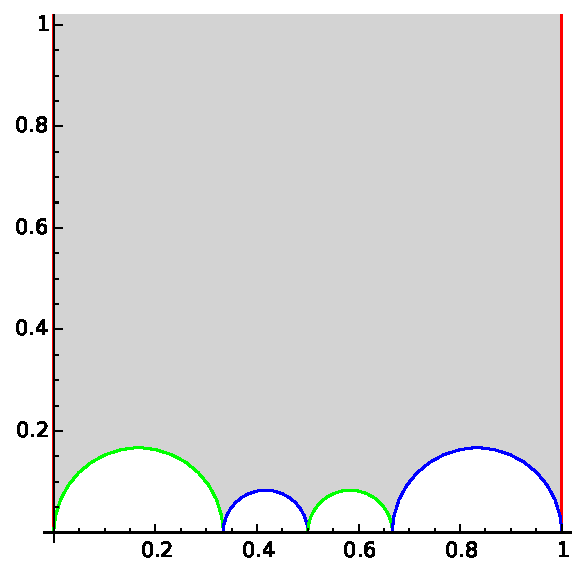
\includegraphics[width=1\linewidth]{X0_11.pdf}
	\caption{$X_0(11)$\label{X0_11.svg}}
	\end{subfigure}
	\begin{subfigure}{.5\linewidth}
	\centering
	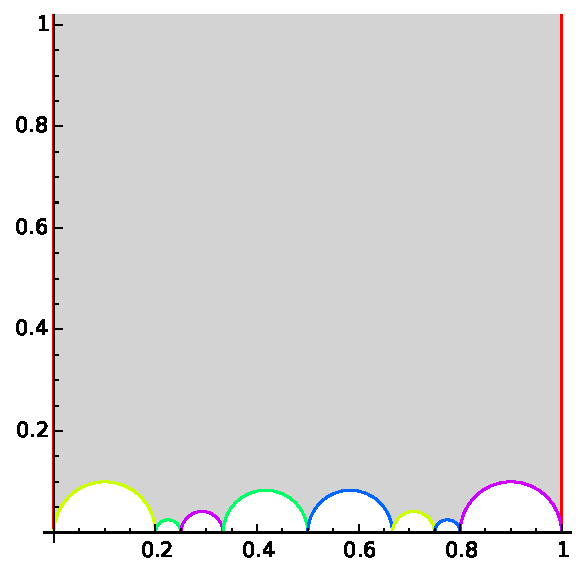
\includegraphics[width=1\linewidth]{X0_23.pdf}
	\caption{$X_0(23)$\label{X0_23.svg}}
	\end{subfigure}
	\caption{Fundamental Domains}\label{fund_domains}
\end{figure}



\section{$X(1)$}

Let $\Lambda$ be a lattice and choose a basis $\free{\omega_1,\omega_2}$. Up to scaling and obvious changes, we can normalize the basis to $\free{\tau,1}$ with $\tau = \frac{\omega_1}{\omega_2}\in\HH$. We denote $\Lambda_\tau$ as the lattice given by $\free{\tau,1}$. However, $\tau$ is not unique (for example $\Lambda_{\tau+1} = \Lambda_\tau$ would give the same lattice). It isn't too hard to figure out exactly how to fix the uniqueness.
\begin{thm}\label{uniquenessoflattices}
	$\Lambda_{\tau} \approx \Lambda_{\tau'}$ if and only if $\tau' = \gamma(\tau)$ for some $\gamma\in\SL_2(\ZZ)$. In which case, $(c\tau+d)\Lambda_{\tau'} = \Lambda_\tau$.
\end{thm}
\begin{proof}
	\hfill
	\begin{enumerate}
		\item[$(\Leftarrow)$:]
			Note $\gamma$ applied to the basis $\{\tau,1\}$ gives $\{a\tau+b,c\tau+d\}$. Because $\gamma\in\SL_2(\ZZ)$ we have $\free{\tau,1} = \free{a\tau+b,c\tau+d}$. Note the ratio of the second basis is $\frac{a\tau+b}{c\tau+d} = \gamma(\tau) = \tau'$. Hence
			$$
			\Lambda_{\tau'} = \free{\tau',1} \approx (c\tau+d)\free{\tau',1} = \free{a\tau+b,c\tau+d} = \free{\tau,1} = \Lambda_\tau.
			$$
		\item[$(\Rightarrow)$:]
			If $\Lambda_{\tau} \approx \Lambda_{\tau'}$ then we can find a number $m$ such that $m\Lambda_{\tau'} = \Lambda_{\tau}$. Then there is a change of basis $\gamma\in\SL_2(\ZZ)$ taking $\free{\tau,1}$ to $\free{m\tau',m}$ (possibly normalizing so determinate is positive). Taking the ratios of the basis gives $\gamma(\tau) = \tau'$.
	\end{enumerate}
\end{proof}

This means we have a bijection between $Y(1)$ and $\script{L}/\CC^\ast$. Combining this result with above, we have the following.

\begin{thm}\label{Y1moduli}
	There is a bijection between points on $Y(1)$ and isomorphism classes of elliptic curves.
\end{thm}

\begin{cor}\label{X1moduli}
	There is a bijection between the non-cusps of $X(1)$ and isomorphism classes of elliptic curves over $\CC$.
\end{cor}

So $X(1)$ is a compact Riemann surface, and hence isomorphic to a projective curve over $\CC$. Most of the points correspond to elliptic curves so it looks like a great candidate for a moduli space. The next obvious question is what curve is $X(1)$?

\subsection{As a Curve}

From the standard fundamental domain, seen in \autoref{X0_1.svg}, it's easy to see there are $3$ distinct vertices, $2$ edges, and $1$ face defining the surface $X(1)$. In the picture in, keep in mind the segment on the imaginary axis in and out of the circle are different. Hence it has genus $0$ and therefore is conformally equivalent to the Riemann sphere, or $\PP^1(\CC)$.

\begin{note}
	In general it is possible to compute the genus of $X_0(N)$ by studying the degree of the obvious map $X_0(N) \to X(1)$. It turns out ramification can only happen at $i,\rho,$ or $\infty$ (i.e. elliptic points and cusps). In \cite[Chapter 5 Section 2]{milne}, Milne references explicit formulas.
\end{note}

\subsection{As a Field}

Recall the $j$-invariant. It can be defined in several ways, but most importantly recall it is a holomorphic function on the upper half plane with a simple pole at $\infty$ (normalized to have residue $1$) and is invariant under $\SL_2(\ZZ)$, i.e. it is a modular function. Hence $j$ descends to a meromorphic function $X(1)\to\PP^1(\CC)$. Because it has one simple pole, general theory of compact Riemann surfaces shows it is conformal. In fact, because we know the automorphisms of $\PP^1(\CC)$ are linear fractional transformations which are uniquely determined by three points, we have proved the following statement.

\begin{thm}
	$j$ is the unique isomorphism $X(1) \to \PP^1(\CC)$ sending $i\mapsto 1728$, $\rho\mapsto 0$, and $\infty\mapsto\infty$.
\end{thm}

\begin{cor}
	The field of meromorphic functions on $X(1)$ is $\CC(j)$.
\end{cor}
\begin{proof}
	This follows from considering the associated map on function fields.
\end{proof}

Note that this shows $X(1)$ can actually be defined over $k$ for any subfield $k\subseteq\CC$, just as $\PP^1(\CC)$ is the same as $\PP^1_{k}(\CC)$ where $\PP^1_k$ is the rational projective line. This follows from a base change from $k$ to $\CC$ which corresponds to field composition $\CC k(j) = \CC(j)$. So we define $X(1)_{k}$ to be $\PP^1_{k}$, i.e. the unique curve with function field $k(j)$. Notice $X(1)_k(\CC) \approx \PP^1_k(\CC) = \PP^1(\CC)$ so this definition makes sense.

The $j$-invariant can be defined completely algebraically based off the coefficients of the elliptic curve. So it still makes sense as a function on elliptic curves over arbitrary fields (though we are only looking at characteristic $0$ right now). So for any such $k$ we have a map
$$
\{E/k\}/\approx ~\to \quad\PP^1_k = X(1)_k
$$
It's looking like we are about to parametrize elliptic curves, but don't get your hopes up.

\begin{fact}
	$X(1)$ is NOT a moduli space for isomorphism classes of rational elliptic curves, i.e. the map above is not bijective (even excluding the cusps), it fails injectivity on non-algebraically closed fields. In particular, the rational points on $X(1)_\QQ$ do not correspond to isomorphism classes of elliptic curves over $\QQ$.
\end{fact}
\begin{reason}
	We know the $j$-invariant works as a parametrization over any algebraically closed field because $E_1\approx E_2$ if and only if $j(E_1) = j(E_2)$. However this does \emph{not} hold if $k$ is not algebraically closed. It is possible for two curves defined over a field $k$ to be isomorphic only over some extension of $k$. But the curves will be isomorphic over a finite extension of $k$ (of degree at most $2$), see Ralph's notes or \cite[Remark II.2.2]{milne}. The most common example is a quadratic twist where we go from $y^2 = x^3 + ax + b$ and $dy^2 = x^3 + ax + b$.
\end{reason}

So close. But what we have isn't useless, we did learn about the $j$-line.


\section{$X_0(N)$}

Next consider the set $S_0$ of pairs $(E,C)$ where $E$ is an elliptic curve over $\CC$ together with a cyclic subgroup of order $N$. We will call two such pairs isomorphic if there is an isomorphism of curves which also identifies the corresponding torsion groups.

\begin{thm}\label{Y_0Nmoduli}
	$X_0(N)$ is a moduli space for $S_0$, i.e. there is a bijection between points on $Y_0(N)$ (the non-cusps of $X_0(N)$) and elliptic curves with an associated cyclic subgroup $C$ of order $N$.
\end{thm}
\begin{proof}
	We will use lattices instead of curves. Let $(\CC/\Lambda,C)\in S_0$. Note that $C$ as a subgroup of $\CC/\Lambda$ can be viewed as a lattice, $\Lambda'\supseteq \Lambda$. As groups, $[\Lambda':\Lambda] = N$. So by the structure theorem of finitely generated groups, we can find a basis $\free{\omega_1,\omega_2}$ for $\Lambda$ such that $\free{\omega_1,\frac{1}{N}\omega_2}$ is a basis for $\Lambda'$. Then by dividing by $\omega_2$ (and possibly normalizing sign), we have shown $(\CC/\Lambda,C) \approx \left(\CC/\Lambda_{\tau},\frac{1}{N}\Lambda\right)$ for some $\tau\in\HH$.

	This gives us a map $S_0 \to Y_0(N)$ sending $\left(\Lambda_\tau,\free{\frac{1}{N}}\right)\mapsto \tau$. It remains to show it's a well defined bijection. Specifically, we need to show if two such pairs are isomorphic if and only if there is some element of $\Gamma_0(N)$ taking one to the other.

	We know from \autoref{uniquenessoflattices} that $\CC/\Lambda_{\tau} \approx \CC/\Lambda_{\tau'}$ if and only if $\tau' = \gamma(\tau)$ for some $\gamma\in\SL_2(\ZZ)$. But now we have extra torsion data, so we want to know which $\gamma$ preserve this as well. Also from \autoref{uniquenessoflattices}, we know $\gamma$ induces the isomorphism $\CC/\Lambda_{\tau'}\to\CC/\Lambda_{\tau}$ given by $z\mapsto (c\tau+d)z$. It remains to check when this isomorphism respects the extra torsion data. This follows by
	$$
	\free{(c\tau+d)\frac{1}{N}\Lambda_{\tau'}} = \free{\frac{c\tau+d}{N}\Lambda_\tau}\equiv\free{\frac{1}{N}\Lambda_\tau}\mod{\Lambda_{\tau}}
	\quad\Leftrightarrow\quad\text{$N\mid c$, i.e. $\gamma\in\Gamma_0(N)$}.
	$$
\end{proof}

\subsection{As a rational curve.}

As before, we will realize $X_0(N)$ as a rational curve by studying its function field. We still have the $j$ function as before. We also have the function $j_N(\tau) = j(N\tau)$. This is a meromorphic function on $X_0(N)$ since
\begin{align*}
	j_N\left(\frac{a\tau+b}{c\tau+d}\right) &= j_N\left(N\frac{a\tau+b}{c\tau+d}\right)
	\\
	&=
	j\left(N\frac{a\tau+b}{c\tau+d}\right)
	\\
	&=
	j\left(\frac{a(N\tau)+Nb}{\frac{c}{N}(N\tau)+d}\right)
	\\
	&=
	j(N\tau) = j_N(\tau).
\end{align*}
Note how we used the hypothesis that $\begin{pmatrix}a&b \\ c &d\end{pmatrix}\in\Gamma_0(N)$ and that $j$ was $\SL_2(\ZZ)$ invariant.

\begin{thm}\label{C(X_0(N))}
	$j$ and $j_N$ generate the meromorphic functions on $X_0(N)$, i.e. $\CC(X_0(N)) = \CC(j,j_N)$. Moreover, the minimal polynomial of $j_N$ over $\CC(j)$ is has coefficents in $\QQ$.
\end{thm}
\begin{proof}(See \cite[Chapter 5 Section 2]{milne}). Sketch:
	Pick coset representatives $\gamma_i$ for $\Gamma_0(N)\backslash\SL_2(\ZZ)$ so $\SL_2(\ZZ) = \bigsqcup \Gamma_0(N)\gamma_i$. Note there are precisely $m = [\SL_2(\ZZ):\Gamma_0(N)]$ representatives. Hence $m = \deg(X_0(N) \to X(1))$ and therefore $m = [\CC(X_0(N)):\CC(X(1))] = [\CC(X_0(N)):\CC(j)]$. So it is enough to find an element of degree $m$ over $\CC(j)$.

	Then the minimal polynomial for $j_N$ over $\CC(j)$ is turns out to be
	$$
	F(j,Y) = \prod \left(Y - j(N\gamma_i\tau)\right)
	$$
	which has degree $m$.

	Note that each term is \emph{not} in $\CC(j)$, but the symmetric polynomial made by the product is actually invariant under $\SL_2(\ZZ)$, so it is infact a rational function in $\CC(j)[Y]$ (since $\CC(X(1)) = \CC(j)$). Because the product is holomorphic on $\HH$, the coefficients must lie in $\CC[j,Y]$.

	One can show $F(j,Y)\in\QQ[j,Y]$ using the fact that $j$ has a rational $q$-expansion, and hence a relation between $j$ and $j_N$ must lie over $\QQ$.
\end{proof}

\begin{cor}
	$\CC(X_0(N)) = \CC\QQ(j,j_N)$.
\end{cor}

This allows us to define $X_0(N)_\QQ$ as the $\QQ$ curve corresponding to the function field $\QQ(j,j_N)$.

\begin{ex}
	In the case of $N = 11$ it is possible to explicitly describe $X_0(11)_\QQ$. The idea is to write down two modular functions $x,y$ for $\Gamma_0(11)$ with a single pole at $i\infty$ of order at most $2,3$ respectively. It follows from Riemann-Roch (see \cite[Chapter II Section 5 Corollary 5.5c]{silverman1}) that $l(D) = \deg D - g + 1$ (with usual notation) so the space of functions with a pole of at most order $6$ at $i\infty$ is exactly $6$. But we have seven functions, $1,x,y,x^2,xy,y^2,x^3$. Hence we get a non-trivial linear relation which when normalized is exactly a Weirstrass equation.

	In \cite[Section 4]{weston}, the author finds such functions $x,y$. The construction of $x,y$ is complicated so we'll skip it. It uses a lot of complex analysis, theta functions, and modular forms. We end up with (after a lot of hard and clever work) is the equation
	$$
	X_0(11)\colon~ y^2 + y = x^3 - x^2 - 10x - 20
	$$
	This gives us an explicit model over $\QQ$ to work with.
\end{ex}

\subsection{Rational Points on $X_0(N)$}

\begin{quest}
	Is $X_0(N)$ a moduli space for elliptic curves over $\QQ$ with Galois invariant subgroups $C$ of $E(\overline{\QQ})$ (meaning $\sigma(C) = C$ for all $\sigma\in\Gal(\overline{\QQ}/\QQ)$) of order $N$?
\end{quest}

First we need to know why did I write ``Galois invariant'' subgroups. This is because given a Galois invariant subgroup $C$ of a rational curve $E$, there exists a rational elliptic curve $E'$ and isogeny $E\to E'$ with kernel $C$. Moreover, $E'$ is unique up to an isomorphism over $\QQ$. For a proof, see \cite[Chaptr III Ex 3.13e]{silverman1}. The idea is to take all the field automorphisms given by translation by elements of $C$ and then take the corresponding fixed field. We denote $E'$ by $E/C$.

Now we have a natural map in one direction.
\begin{equation}\label{eq:X_0jmap}
(E,C) \mapsto (j(E),j(E/C))
\end{equation}

Where the right hand side is a point on the curve $\script{C}_N$ given by the equation $\QQ[x,y]/F(x,y)$ where $F$ is the same function as in the proof of \autoref{C(X_0(N))}. To show this map makes sense we have to check the following.

\begin{prop}
	$j(E/C) = j_N(E)$
\end{prop}
\begin{proof}
	If $(E,C)$ is represented by $\left(\CC/\Lambda_{\tau},\free{\frac{1}{N}}\right)$ then $E/C$ corresponds to the lattice spanned by $\{\tau,\frac{1}{N}\}$ which we can scale to get the lattice spanned by $\Lambda_{N\tau} = \{N\tau,\frac{1}{N}\}$. Hence $E/C \cong \CC/\Lambda_{N\tau}$ so $j(E/C) = j(N\tau) = j_N(E)$.
\end{proof}

\begin{rem}
While $\script{C}_N$ gives us an equation for $X_0(N)$ (hence a model for $X_0(N)_{\QQ}$), in practice it is difficult to compute explicitly.
\end{rem}

\begin{ex}
	Let $E$ be the curve $y^2 = x^3 - x$ which has $j$-invariant $1728$. Let $P$ be the point $(x,y)=(-1,0)$ of order $2$. Then with sage we can compute the isogenous curve given by $E/\free{P}$.
\begin{sagecode}
	\begin{sagecell}
E1 = EllipticCurve([0,0,0,-1,0])
phi = EllipticCurveIsogeny(E1,E1.torsion_points(2)[0])
E2 = phi.codomain(); E2
E2.j_invariant()
	\end{sagecell}
	\begin{sageout}
Elliptic Curve defined by y^2 = x^3 - 11*x + 14 over Rational Field
287496
	\end{sageout}
\end{sagecode}
	\noindent To see this is indeed the right map, we can enter
\begin{sagecode}
	\begin{sagecell}
phi.kernel_polynomial()
phi.degree()
	\end{sagecell}
	\begin{sageout}
x + 1
2
	\end{sageout}
\end{sagecode}
\end{ex}

In general, the map in \autoref{eq:X_0jmap} is not surjective as we will see later due to Mazur's Theorem.

\begin{ex}
	Recall the equation for $X_0(11)$ is $y^2 + y = x^3 - x^2 - 10x - 20$. In sage we can compute
\begin{sagecode}
\begin{sagecell}
E = EllipticCurve([0,-1,1,-10,-20]); E
\end{sagecell}
\begin{sageout}
Elliptic Curve defined by y^2 + y = x^3 - x^2 - 10*x - 20 over Rational Field
\end{sageout}
\begin{sagecell}
E.rank()
\end{sagecell}
\begin{sageout}
0
\end{sageout}
\begin{sagecell}
E.torsion_order()
\end{sagecell}
\begin{sageout}
5
\end{sageout}
\end{sagecode}

	Thus $X_0(11)$ has $5$ rational points. One can show as an exercise that $[\SL_2(\ZZ):\Gamma_0(p)] = p+1$. This means the degree of the map $X_0(11) \to X(1)$ is $12$ and hence there are $12$ cusps counting multiplicity. In fact it turns out there is only $2$ actual cusp points. These do not correspond to elliptic curves because remember the map in \autoref{eq:X_0jmap} lands in $Y_0(N)$. We can not say what exactly the other $3$ points mean, so for now they just mean we need a better space.
\end{ex}

The following theorem shows how close $X_0(N)$ is to a fine moduli space.

\begin{thm}
	The map in $\autoref{eq:X_0jmap}$ is functorial in $k$ and always surjective onto $Y_0(N)_k$ for any field $k$ of characteristic $0$. When $k$ is algebraically closed it is a bijection.
\end{thm}
\begin{proof}
	See \cite[Chapter V Theorem 2.7]{milne}.
\end{proof}

\section{$X_1(N)$}

Next consider the set $S_1$ of pairs $(E,P)$ where $E$ is an elliptic curve over $\CC$ and $P$ is a point of order $N$.

\begin{thm}
	$X_1$ is a moduli space for $S_1$, i.e. there is a bijection between points on $Y_1(N)$ and elliptic curves with associated point $P$ of order $N$.
\end{thm}
\begin{proof}
	This should follow similarly to \autoref{uniquenessoflattices} and \autoref{Y_0Nmoduli}.

	The first step is to show any pair $\left(\CC/\Lambda,w\right)$ is isomorphic to a pair $\left(\CC/\Lambda_\tau,\frac{1}{N}\right)$ for some $\tau$.

	\noindent
	From the proof of \autoref{Y_0Nmoduli} we know such a pair is isomorphic to $\left(\CC/\Lambda_\tau,\frac{c\tau+d}{N}\right)$ for some $\tau$ and $c,d\in\ZZ$.

	Now by hypothesis the point $\frac{c\tau+d}{N}$ must have order exactly $N$. Another way to say this is $(\overline{c},\overline{d})$ has order $N$ in $\ZZ/N\ZZ\times\ZZ/N\ZZ$ where $\overline{c}$ is the reduction of $c$ modulo $N$. This means $\gcd(\overline{c},\overline{d}) = 1$ so we can find $a,b\in\ZZ$ such that $ad - bc \equiv 1 \mod{N}$, i.e. the matrix $\gamma = \begin{pmatrix}a&b\\c&d\end{pmatrix}\in M_2(\ZZ)$ descends to $\SL_2(\ZZ/N\ZZ)$. Modifying the matrix modulo $N$ (i.e. adding multiples of $N$ to the entries) preserves the point $\frac{c\tau+d}{N}$ so we may choose $\gamma\in\SL_2(\ZZ)$. This is because the map $\SL_2(\ZZ) \to \SL_2(\ZZ/N\ZZ)$ is surjective. Define $\tau' = \gamma(\tau)$ and notice the isomorphism $\CC/\Lambda_{\tau'} \to\CC/\Lambda_\tau$ is given by multiplication by $c\tau+d$ and hence takes the point $\frac{1}{N}$ to $\frac{c\tau+d}{N}$.

	The next step is to show
	$$
	\left(\CC/\Lambda_\tau,\frac{1}{N}\right) \approx \left(\CC/\Lambda_{\tau'},\frac{1}{N}\right)
	\quad\Leftrightarrow\quad
	\tau'=\gamma(\tau) \quad\text{ for some $\gamma\in\Gamma_1$}.
	$$
	\begin{enumerate}
		\item[$(\Leftarrow)$:]
			We know there is an isomorphism $\Lambda_{\tau'} \to\Lambda_{\tau}$ given by multiplication by $c\tau+d$. Note by definition of $\Gamma_1$ we have
			$$
			\frac{1}{N} \mapsto (c\tau+ d)\frac{1}{N} \equiv \frac{1}{N} \mod{\Lambda_\tau}
			$$
			because $c\equiv 0\mod{N}$ and $d\equiv 1\mod{N}$.

		\item[$(\Rightarrow)$:]
			We can apply the same reasoning as in \autoref{uniquenessoflattices} to find some $\gamma\in\SL_2(\ZZ)$ which must induce the isomorphism $\left(\CC/\Lambda_{\tau'},\frac{1}{N}\right) \to \left(\CC/\Lambda_{\tau},\frac{1}{N}\right)$. By hypothesis we have then that $(c\tau+d)\frac{1}{N} \equiv \frac{1}{N}\mod{\Lambda_{\tau}}$. This implies $c\equiv 0\mod{N}$ and $d\equiv 1\mod{N}$ which is enough as the condition on $a$ is forced by looking at the determinate formula modulo $N$.
	\end{enumerate}
\end{proof}

\subsection{As a Rational Curve}

Arguments a little more complicated but similar to those in we used for $X_0(N)$ show that $X_1(N)$ is again a rational curve. There is still a natural map $S_1 \to Y_1(N)$ over $\QQ$.

\subsection{$X_1(11)$}

\begin{fact}
	$X_1(11)_{\QQ}$ is a fine moduli space (after accounting for cusps as usual) for rational elliptic curves with a given point of order $11$.
\end{fact}

The proof is difficult but the main reason why $X_1(11)$ works and $X_0(11)$ did not is because of something someone might call ``rigidity''. Two rational elliptic curves with given Galois invariant subgroups of order $N$ can be isomorphic over $\overline{\QQ}$ but not over $\QQ$ as we saw above. This is because of the variety of isomorphisms, which can be viewed as ``twists'' of points on $X_0(11)$.

It turns out that $X_1(N)$ is more rigid. Between any two pairs $(E,P)$ and $(E',P')$ there is at most one isomorphism $E\to E'$ sending $P$ to $P'$. Assuming this fact, note that given such an isomorphism $\varphi:E\to E'$ we can choose any $\sigma\in\Gal(\overline{\QQ}/\QQ)$ and look at $\varphi^{\sigma}:E^{\sigma}\to (E')^{\sigma}$, meaning apply $\sigma$ to all the coefficients. Because $E,E',P,P'$ are all rational they stay the same and hence by rigidity $\varphi^\sigma = \varphi$ and hence $\varphi$ is defined over $\QQ$.

This doesn't prove it is a fine moduli space, but it does show that the big obstruction for $X_0(11)$ and $X(1)$ doesn't exist for $X_1$.

\subsubsection{Points}

First with some combinatorial algebra, one can show $X_1(11)_{\QQ}$ has $5$ cusps. It is not hard to show $X_1(11)$ has $10$ cusps, but then it turns out they are not all ``rational''. So there are only $5$ cusps on $X_1(11)_{\QQ}$. These are points on $X_1(11)$ which do not correspond to rational curves in $S_1/\QQ$.

We (or somebody very comfortable with modular forms and theta functions) can again somehow calculate a model for $X_1(11)$ as we did for $X_0(11)$. It turns out to be
$$
	X_1(11): ~ y^2 + y = x^3 - x^2
$$
Now we can plug this into sage and note
\begin{sagecode}
\begin{sagecell}
E = EllipticCurve([0,-1,1,0,0]); E
\end{sagecell}
\begin{sageout}
Elliptic Curve defined by y^2 + y = x^3 - x^2 over Rational Field
\end{sageout}
\begin{sagecell}
E.rank()
\end{sagecell}
\begin{sageout}
0
\end{sageout}
\begin{sagecell}
E.torsion_order()
\end{sagecell}
\begin{sageout}
5
\end{sageout}
\end{sagecode}

Thus we have just shown that \emph{no} rational elliptic curves have a point of order $11$. What is even more remarkable, is that Mazur showed $X_1(N)$ fails to have rational points for almost all $N$. This gave the following theorem.

\begin{thm}[Mazur's Torsion Theorem (1977)]
	Let $E$ be an elliptic curve over $\QQ$. Then the torsion subgroup of $E(\QQ)$ if one of the following $15$ groups:
	\begin{enumerate}
		\item[$(1-11)$:] $\ZZ/N\ZZ$ for $N = 1,2,3,4,5,6,7,8,9,10,12$.
		\item[$(12-15)$:] $\ZZ/2\ZZ\times\ZZ/N\ZZ$ for $N=1,2,3,4$.
	\end{enumerate}
\end{thm}



\bibliographystyle{alpha}
\bibliography{references}


\begin{center}
\noindent\rule{4cm}{.5pt}
\vspace{.25cm}

\noindent {\sc \small \myauthor}\\
{\small Department of Mathematics, University of Washington, Seattle WA 98195} \\
email: {\tt \myemail}
\end{center}

\end{document}